\documentclass[uplatex, 11pt,a4j, titlepage]{jsarticle}

\usepackage{assets/preamble}
\usepackage{assets/info}
\usepackage{listings,jlisting}

% Title
\title{DC サーボモータと制御系}
\date{\today}
\author{
    \small{\myid} \\
    \myname\thanks{\mymail}
}

\begin{document}
\maketitle

% 実験レポート1
% ここから

\subtitle{2020/10/9}

\theme{実験1}
\section{目的}
DCサーボモータの周波数応答の測定を元に伝達関数を同定する。
ここで、制御対象としてのDCサーボモータにはドライバやタコジェネレータ、
ポテンショメータを制御対象として含む。
周波数応答測定に基づく同定を通して動的システムの周波数特性に親しむ。
\section{原理}
DCサーボモータは図\ref{dc_eq}のような等価回路で表現できる。
$e(t)$は電機子に誘起される逆起電力なので、印加される電圧$v(t)$、
電機子に流れる電流$i(t)$、電機子の抵抗$R$、インダクタンス$L$に対して
次式が成立する。

\begin{equation}\label{one}
    v(t) = Ri(t) + L\frac{\rm d}{{\rm d}t}i(t) + e(t)
\end{equation}

また、電機子の回転速度を$\omega (t)$とすると、
比例定数を$k_{\rm E}$として逆起電力に比例するので

\begin{equation}\label{two}
    e(t) = k_{\rm E} \omega (t)
\end{equation}

が成立する。
また電機子に作用する回転トルク$\tau (t)$をすると、
比例定数を$k_{\rm T}$として電機子電流に比例するので

\begin{equation}\label{three}
    \tau (t)=k_{\rm T} i(t)
\end{equation}

が成立する。

ここで、電機子の慣性モーメントを$J$、負荷トルクを$\tau_{\rm L}$、
電機子の回転に関する粘性摩擦係数を$D$とすると運動方程式より

\begin{equation}\label{four}
    \tau (t) - \tau_{\rm L}(t)
        = J \frac{\rm d}{{\rm d}t} \omega (t) + D\omega(t)
\end{equation}

が成立する。ここで、式\ref{one}、\ref{two}、\ref{three}、\ref{four}
をそれぞれラプラス変換すると

\begin{equation}\label{five}
    V(s) = RI(s) + sLI(s) + E(s)
\end{equation}

\begin{equation}\label{six}
    E(s) = k_{\rm E} \Omega (s)
\end{equation}

\begin{equation}\label{seven}
    T(s) = k_{\rm T}I(s)    
\end{equation}

\begin{equation}\label{eight}
    T(s) - T_{\rm L}(s) = sJ\Omega(s) + D\Omega(s)
\end{equation}

となる。よってこれらの式から$I(s)$、$E(s)$、$T(s)$を消去し、
また電気的時定数$T_{\rm E} = L/R$、
機械的時定数$T_{\rm M}=JR/k_{\rm E}k_{\rm T}$を用いて近似すると

\begin{equation}\label{thirteen}
    \Omega(s)=\frac{1/k_{\rm E}}{(1+sT_{\rm M})(1+sT_{\rm E})}
\end{equation}

が得られる。
したがって印加電圧と回転速度の間の伝達関数は近似的に
二次遅れ系で表現できる。

ここで回転角$\Theta(t)$に対して

\begin{equation}\label{fifteen}
    \Omega(s) = s \Theta (s)
\end{equation}

が成立するはずなので、式\ref{thirteen}より、

\begin{equation}\label{sixteen}
    \Theta(s) = \frac{1/k_{\rm E}}{s(1+sT_{\rm M})(1+sT_{\rm E})}V(s)
\end{equation}

が成立するので、したがって電機子印加電圧と回転角の間の伝達関数$P(s)$は

\begin{equation}\label{seventeen}
    P(s) =\frac{1/k_{\rm E}}{s(1+sT_{\rm M})(1+sT_{\rm E})} 
\end{equation}

とわかる。

今回の制御では検出器をしてタコジェネレータとポテンショメータを用いる。
タコジェネレータの外部端子間に生じる起電力を検出信号$y_{\rm d}$として
測定するので、回転速度と検出信号には

\begin{equation}\label{eighteen}
    y_{\rm d}(t)=k'_{\rm E}\omega(t)
\end{equation}

が成立する。$k'_{\rm E}$は逆起電力定数である。
また、ポテンショメータは回転角に応じて変化する可変抵抗なので、
$k_{\rm P}$を定数としてポテンショメータの検出信号は

\begin{equation}\label{ninteen}
    y_{\rm d}(t) = k_{\rm P}\theta(t)
\end{equation}

となる。

今回の制御では、速度制御ではタコジェネレータ、
位置制御ではポテンショメータからフィードバックすることで
それぞれ図\ref{pv}、図\ref{p}のようなブロック線図で表現できる
フィードバック制御を行う。
制御対象にはDCサーボモータ、ドライバ、操作器が含まれるので、
速度制御に対応する制御対象の伝達関数を$P_{\rm V}(s)$、
位置制御に対応する制御対象の伝達関数を$P(s)$とするとそれぞれ

\begin{equation}\label{twentythree}
    P(s) =\frac{k_{\rm A}k'_{\rm E}/k_{\rm E}}{(1+sT_{\rm M})(1+sT_{\rm E})} 
\end{equation}

\begin{equation}\label{twentyfour}
    P(s) =\frac{k_{\rm A}k_{\rm P}/k_{\rm E}}{s(1+sT_{\rm M})(1+sT_{\rm E})} 
\end{equation}

となる。

\begin{figure}[h]
    \centering
    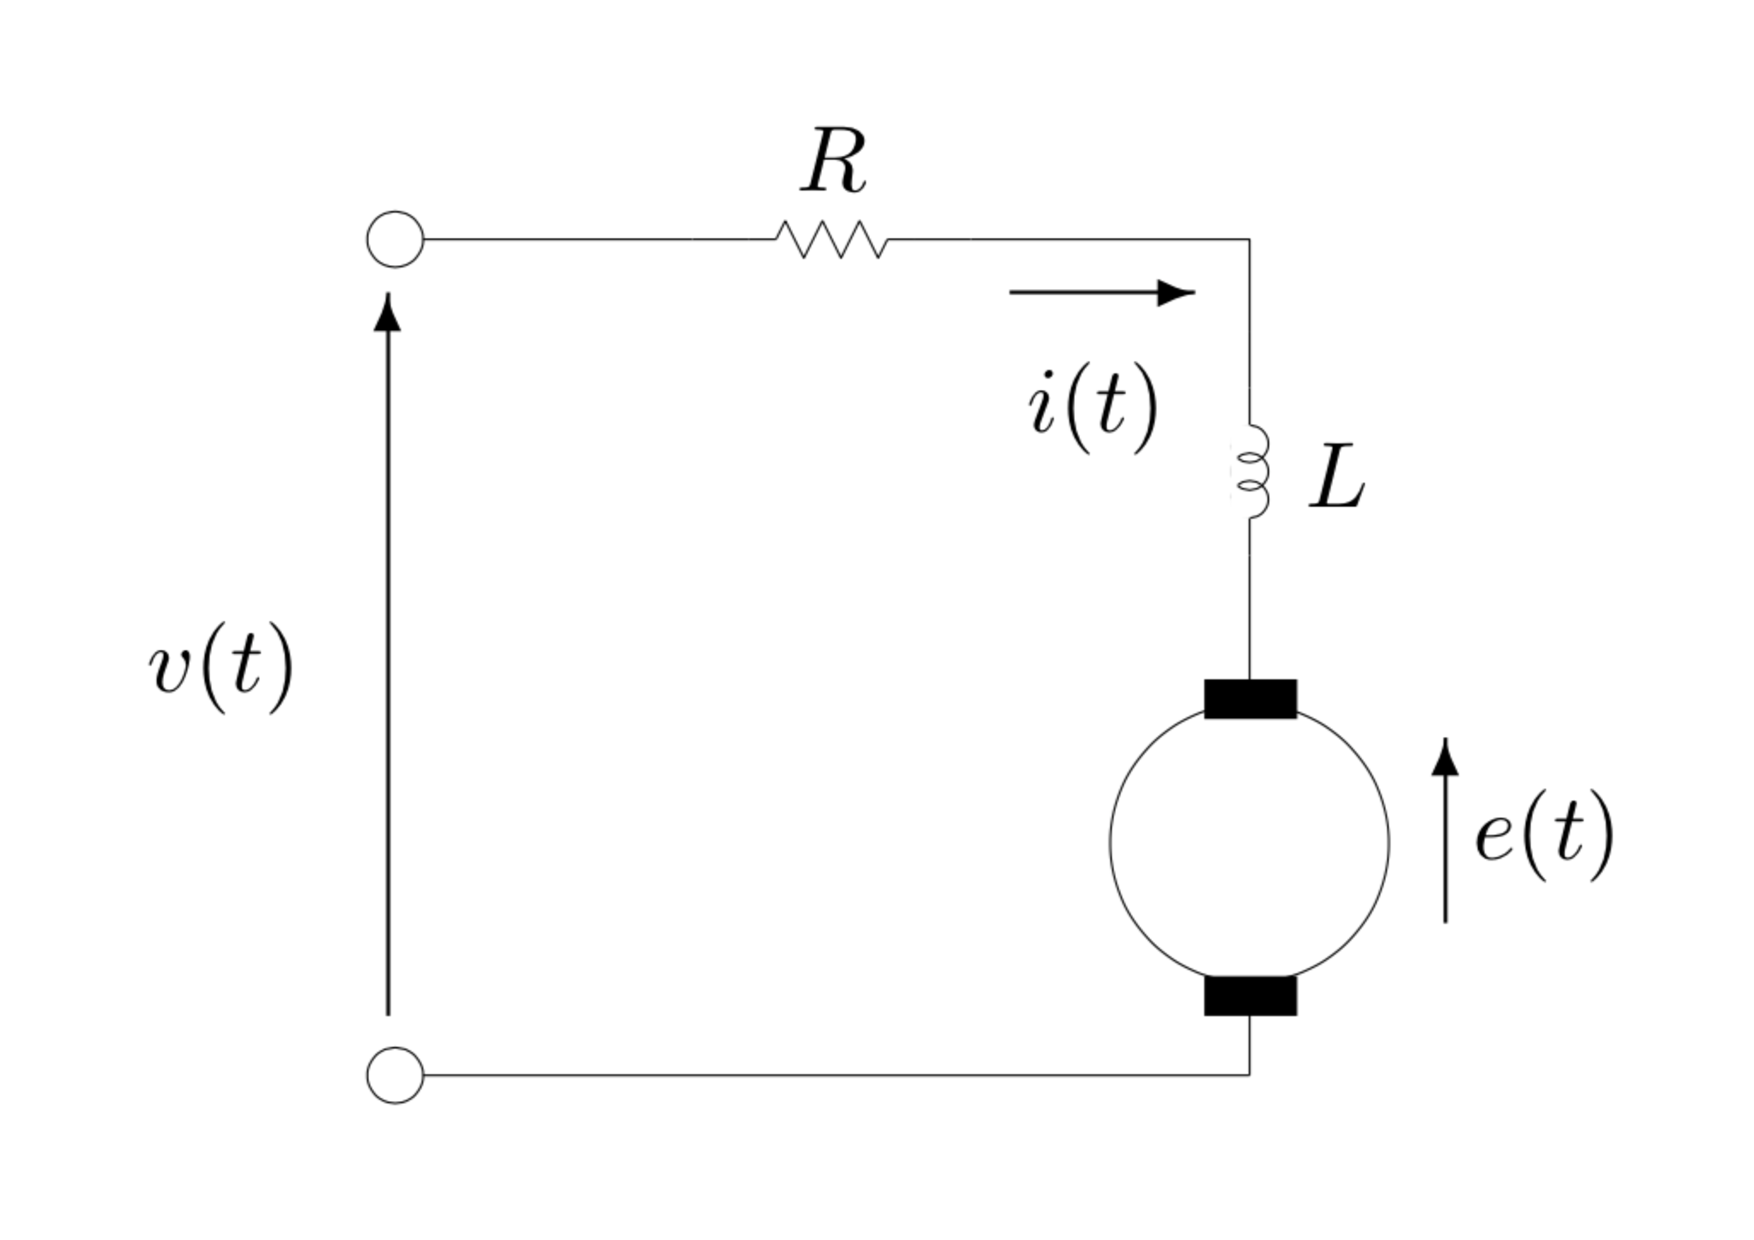
\includegraphics[width=12cm]{dc_eq.pdf}
    \caption{DCサーボモータの等価回路}
    \label{dc_eq}
\end{figure}


\begin{figure}[h]
    \centering
    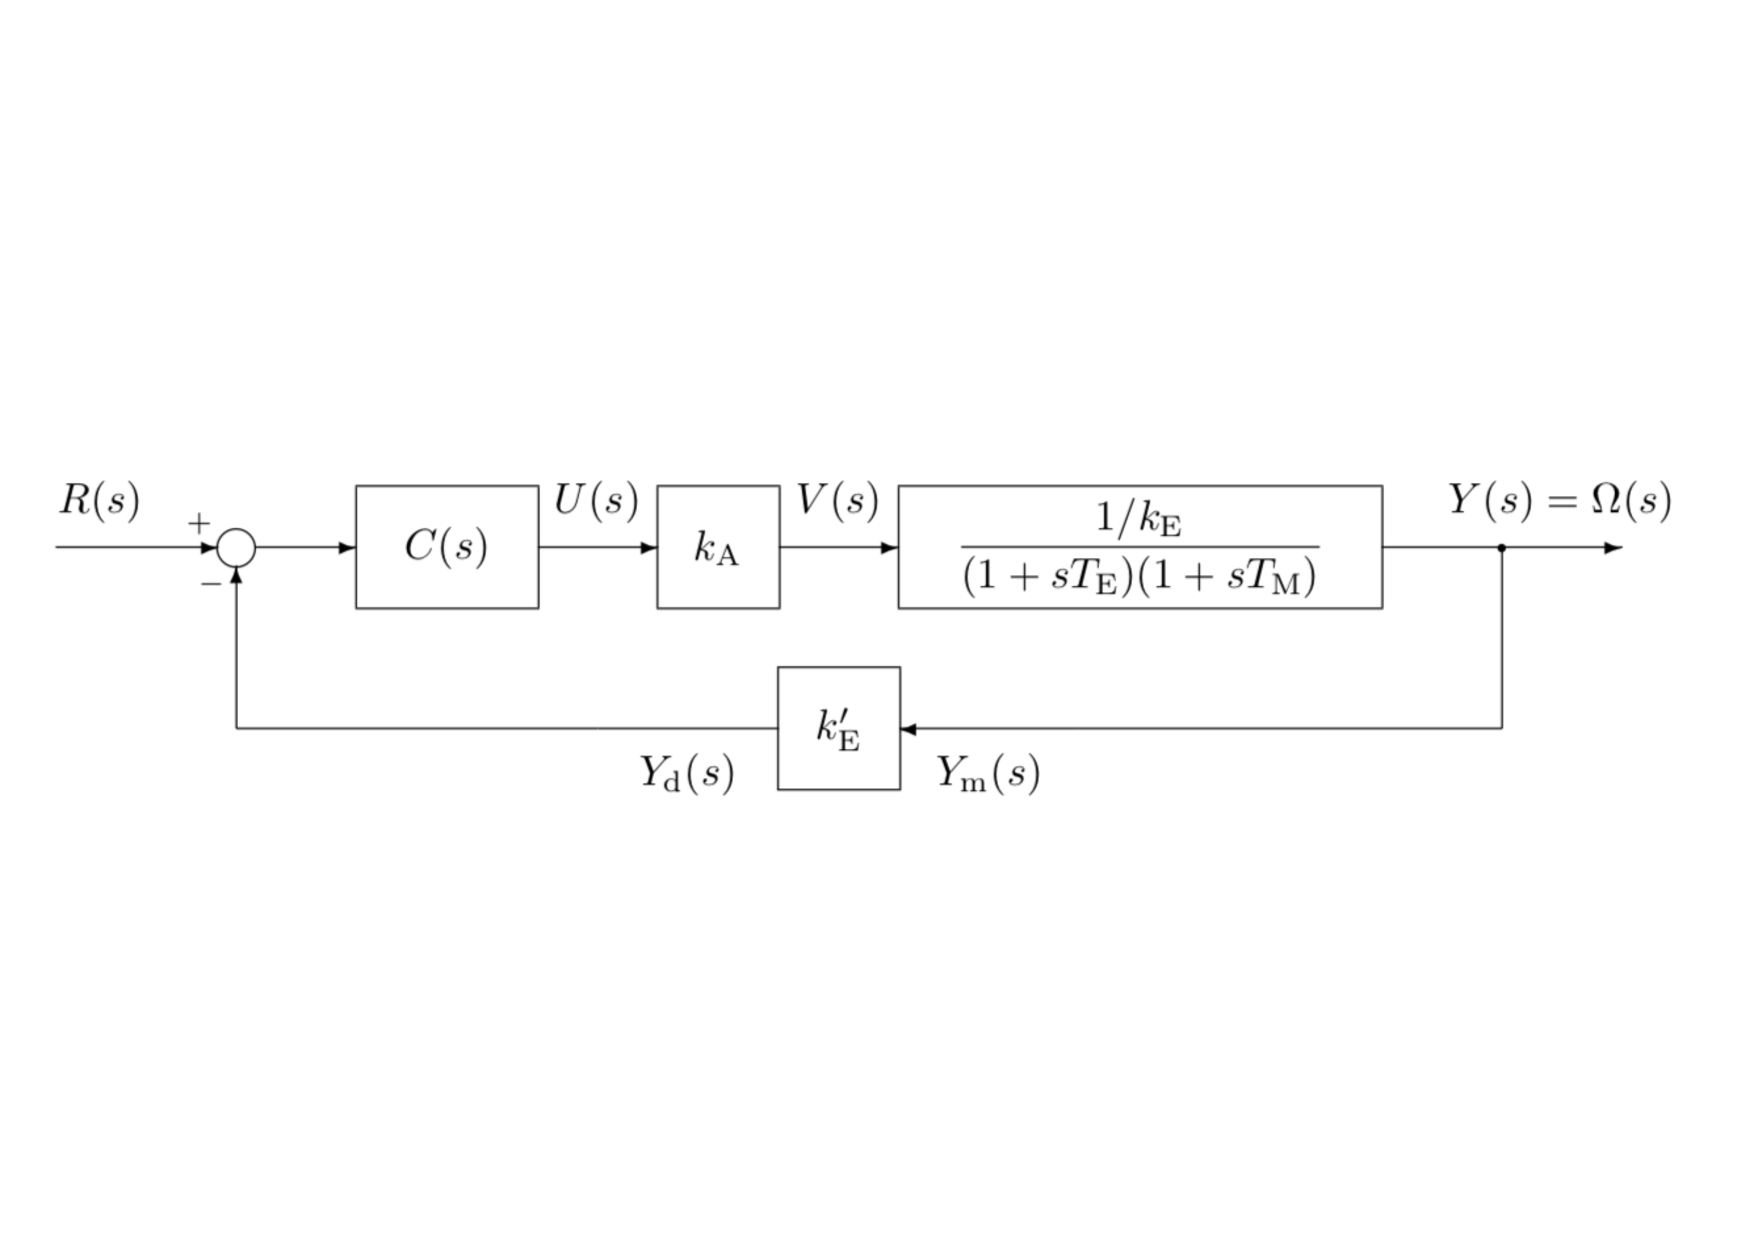
\includegraphics[width=12cm]{pv.pdf}
    \caption{速度制御のブロック線図}
    \label{pv}
\end{figure}

\begin{figure}[h]
    \centering
    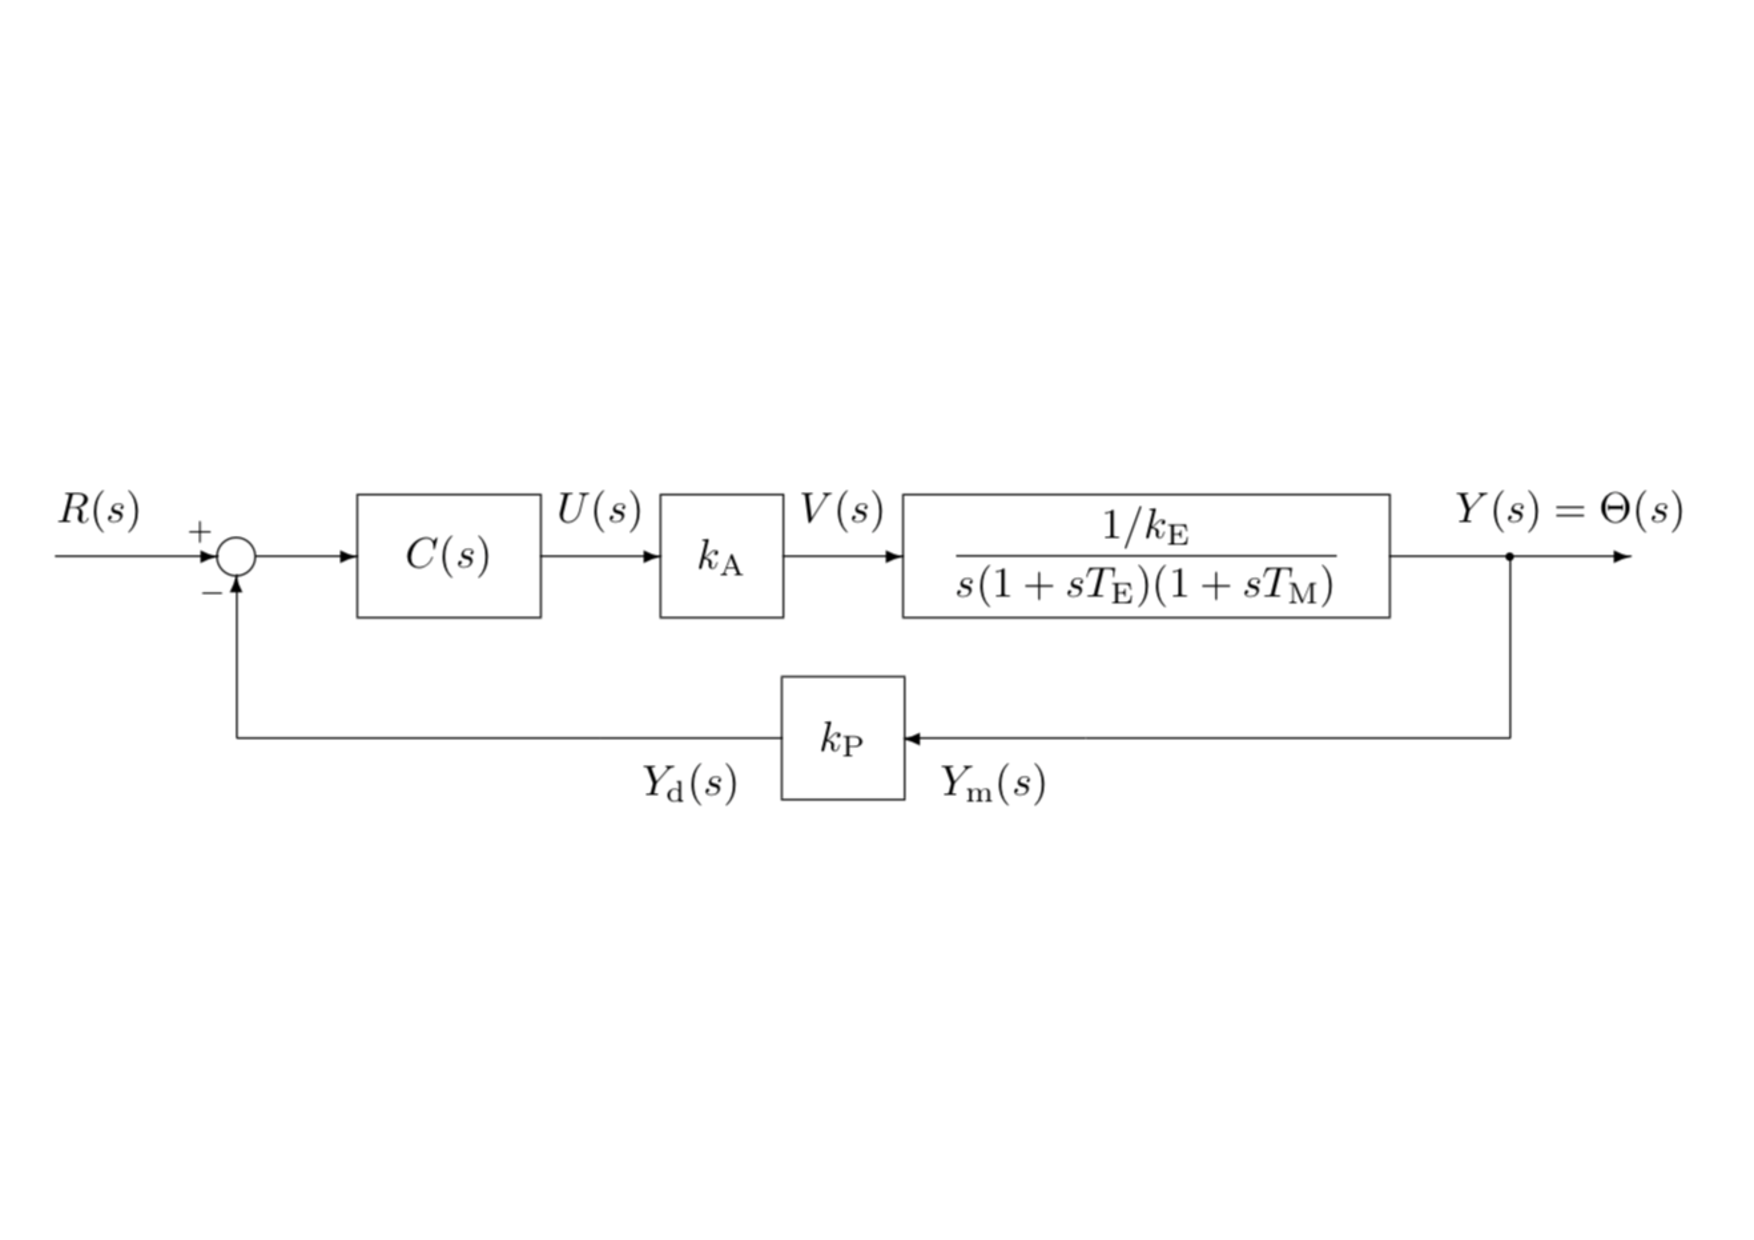
\includegraphics[width=12cm]{p.pdf}
    \caption{位置制御のブロック線図}
    \label{p}
\end{figure}

\newpage 
\ 
\newpage 
\section{方法}

今回用いた器具を以下に示す。

\begin{quote}
    \begin{itemize}
        \item ファンクションジェネレータ:Z94575
        \item オシロスコープ:IWATSU DS-5110 B
        \item 電源(小):KENWOOD PR18-1.2A
        \item 電源(大):TEXIO PS40-10A (Z000323513)
        \item ブレッドボード:5番
        \item DCサーボ:5番
        \item サーボモータドライバ:MS100T05
        \item ポテンショメータ:J40S
        \item カップリング:アサ電子工業製
        \item コンバータ:SUW3 0515
    \end{itemize}
\end{quote}

今実験に用いた装置構成図を図\ref{fig1}および図\ref{fig2}に示す。
図\ref{fig1}は速度制御を行うとき、
図\ref{fig2}は位置制御を行うときに用いた。


\begin{figure}[h]
    \centering
    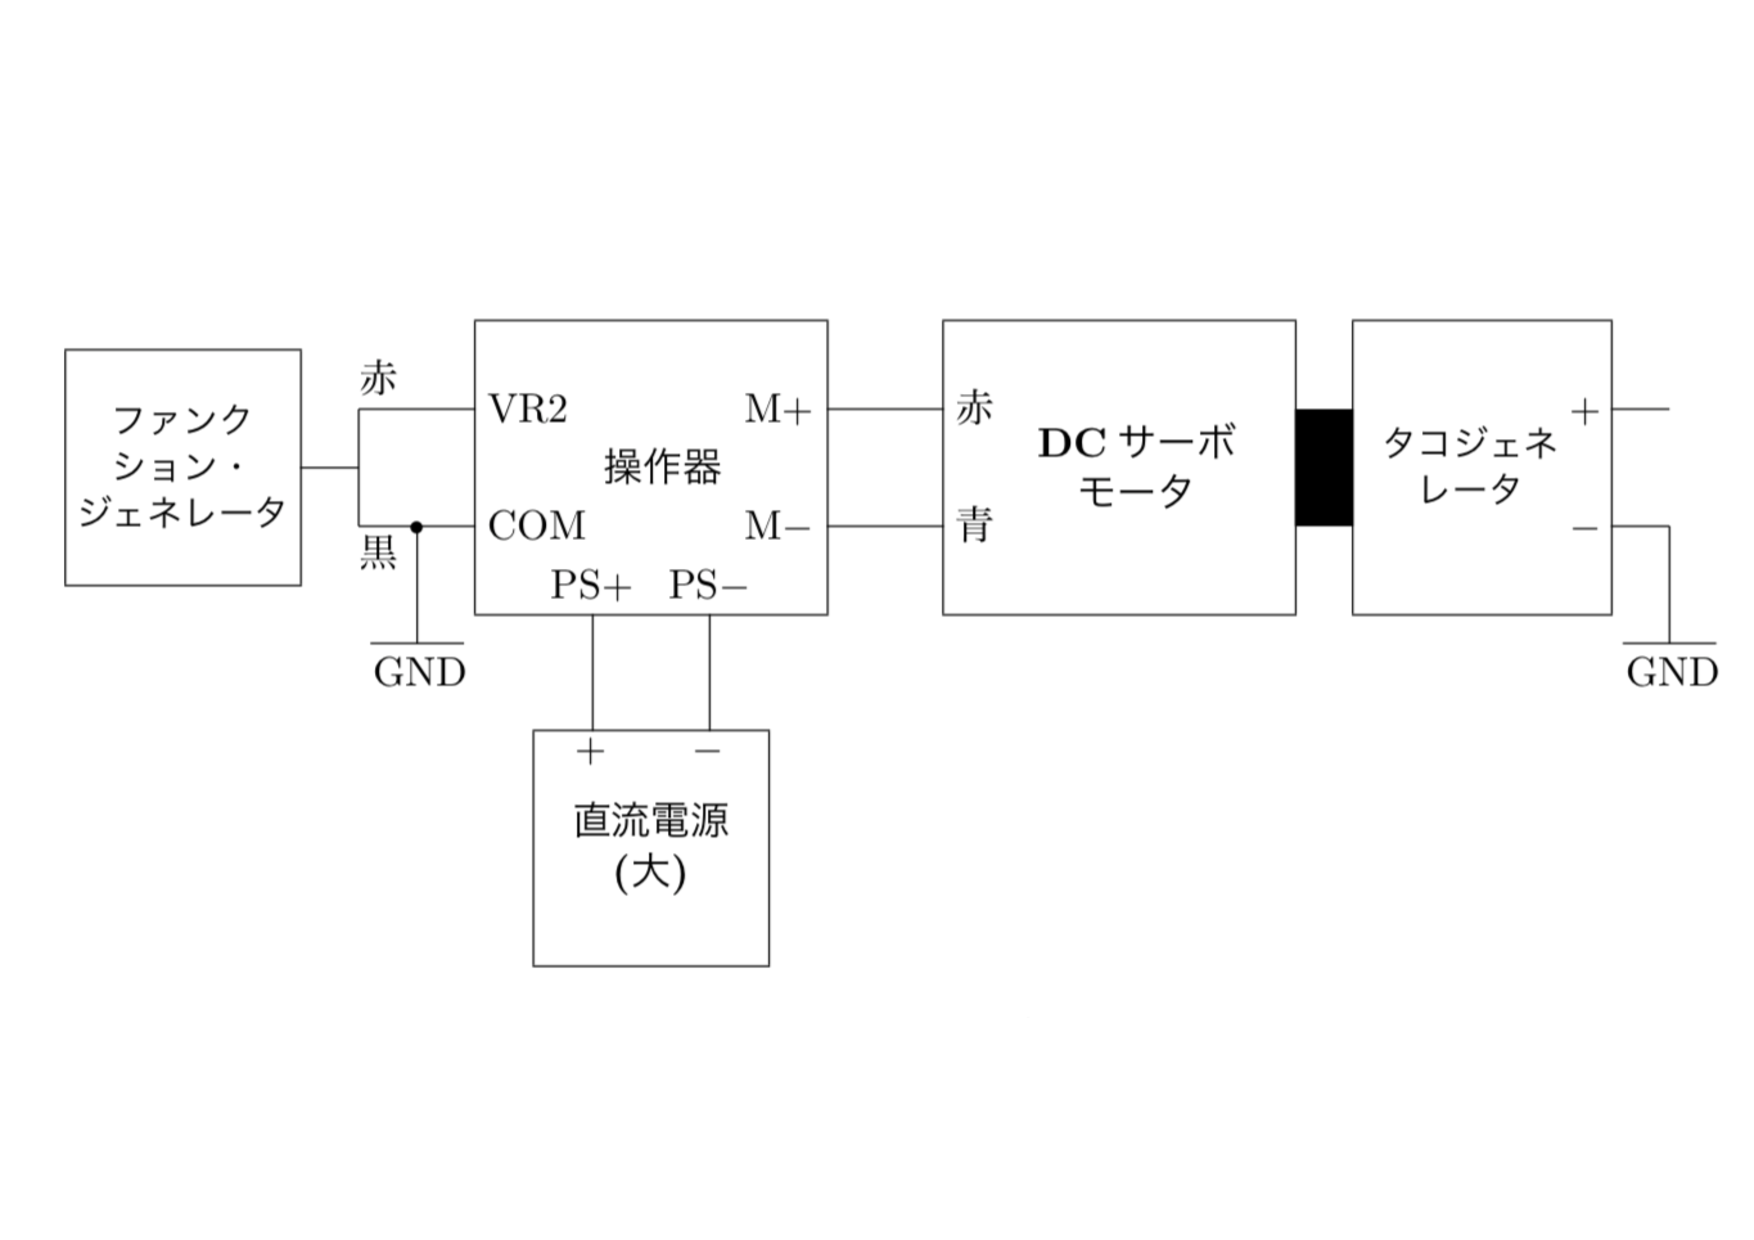
\includegraphics[width=12cm]{fig1.pdf}
    \caption{実験1-1の装置構成図}
    \label{fig1}
\end{figure}

\begin{figure}[h]
    \centering
    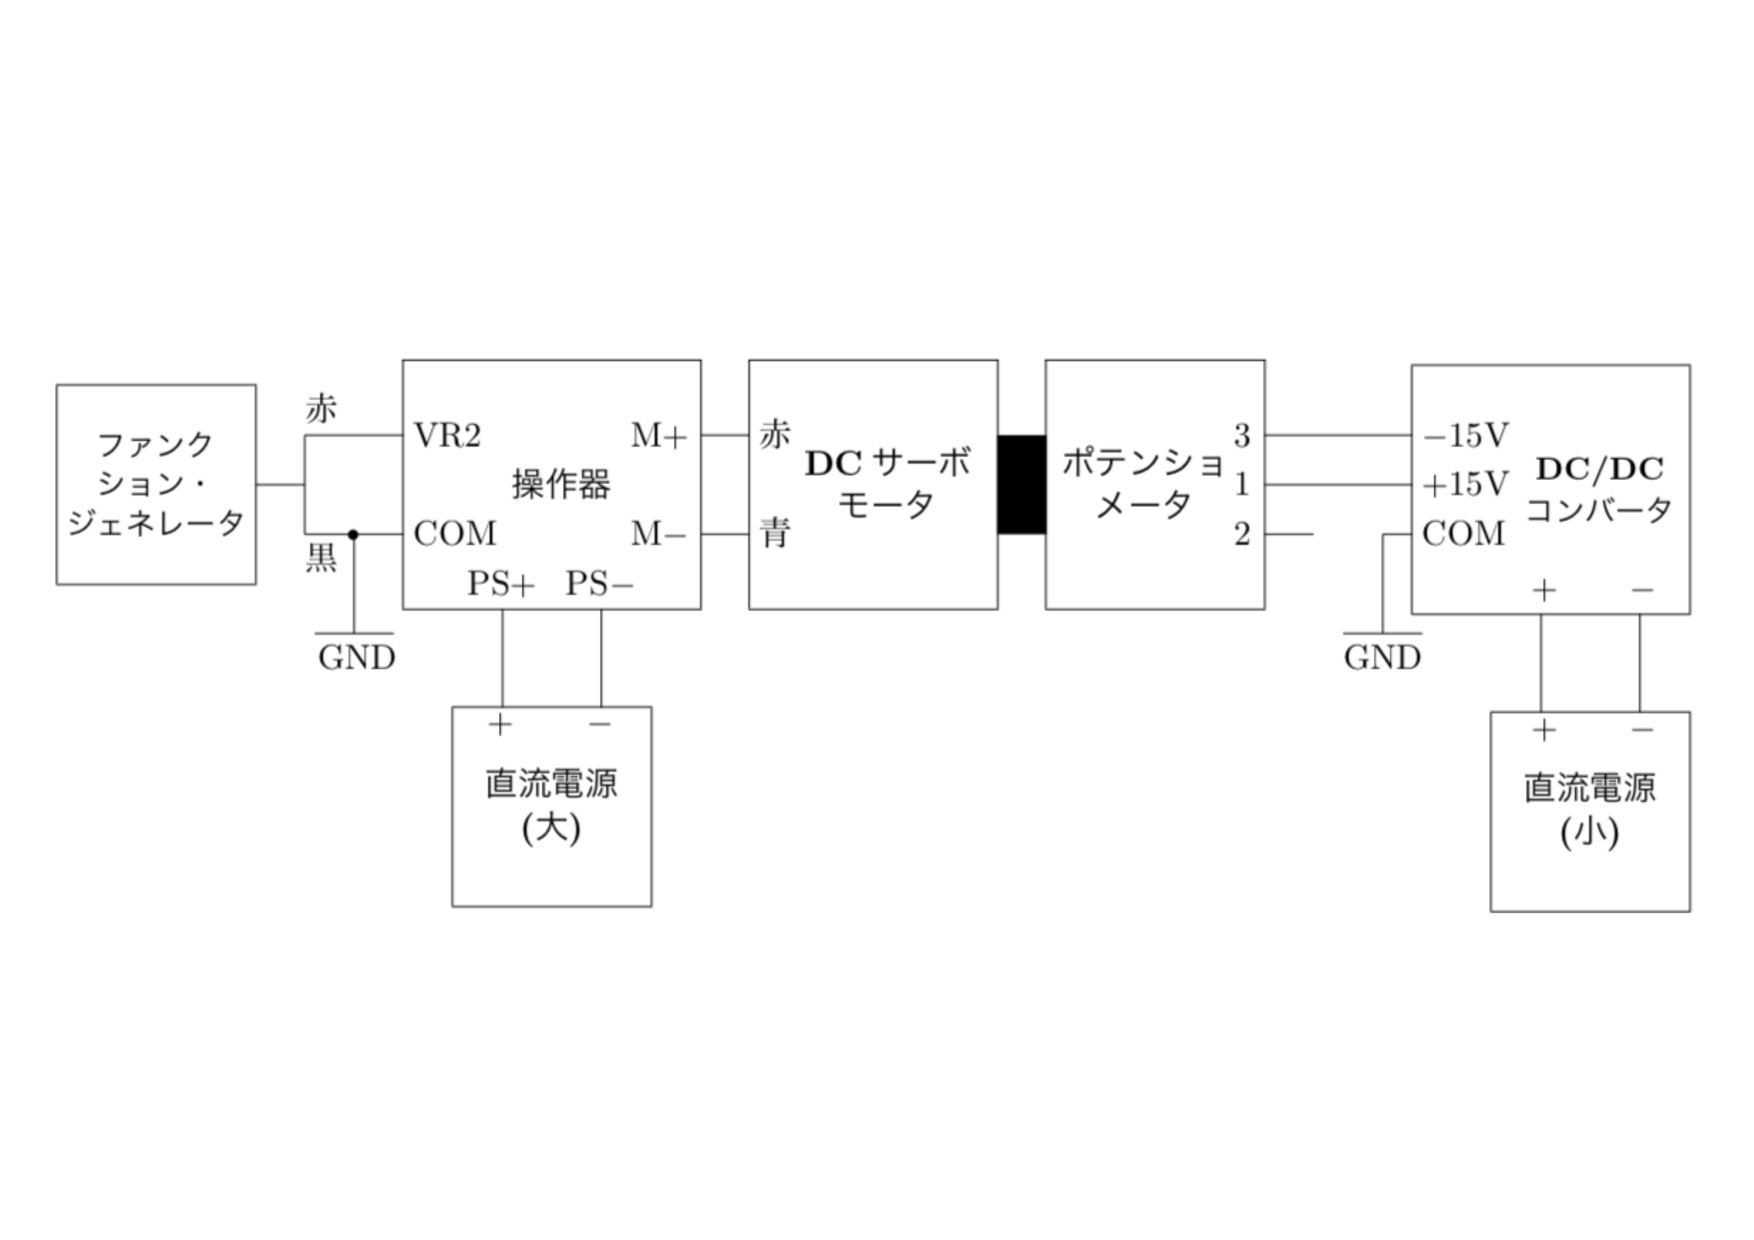
\includegraphics[width=12cm]{fig2.pdf}
    \caption{実験1-2の装置構成図}
    \label{fig2}
\end{figure}

\section{実験結果}
\section{考察}
\section{課題}

% 実験レポート1
% ここまで

\newpage
\resetcounters

% 実験レポート2
% ここから

\subtitle{2020/10/16}

\theme{実験2}
\section{目的}
\section{実験}
\section{実験結果}
\section{考察}
\section{課題}

% 実験レポート2
% ここまで

\newpage
\resetcounters


% 実験レポート3
% ここから

\subtitle{2019/*/*}

\theme{実験3}
\section{目的}
\section{実験}
\section{実験結果}
\section{考察}
\section{課題}

% 実験レポート3
% ここまで

% 参考文献
\newpage
\thispagestyle{empty}
\nocite{Material}
\bibliographystyle{junsrt}
\bibliography{assets/ref}

\end{document}